\documentclass[a4j,twocolumn]{jarticle}
\usepackage[utf8]{inputenc}
\usepackage[cmex10]{amsmath}
\usepackage{amssymb,verbatim}
\usepackage[dvipdfmx]{graphicx}
\usepackage{mathrsfs}
\usepackage{here}
\usepackage{tabularx}

\usepackage{geometry}
\geometry{left=20mm,right=20mm,top=20mm,bottom=20mm}
\fontsize{14pt}{10pt}\selectfont
\def \figref #1{\figurename\ref{#1}}
\def \tbref #1{\tablename\ref{#1}}
\def \equref #1{式(\ref{#1})}
%\vspace{-20cm}
\title{\vspace{-2em}B19 Y00量子暗号のシミュレーション\\
\vspace{0.5cm}
\normalsize{Numerical simulation of ISK-Y00 Cipher}}
\date{}
\pagestyle{empty}
\author{量子情報数理研究室\hspace{50mm}酒寄 遥}
\begin{document}
\maketitle
\thispagestyle{empty}
\section{はじめに}
本論文では,Y00-量子暗号のシミュレーションシステムを用いて減衰通信路に対して,正規受信者の誤り率を評価する.そのとき,受信者側の最大信号強度の設定値を送信者側と一致させる場合と,受信者側の最大信号強度の設定値を減衰の効果を考慮して決める場合を比較する.
\section{光の状態
}
\begin{figure}[htbp]
        \centering   
        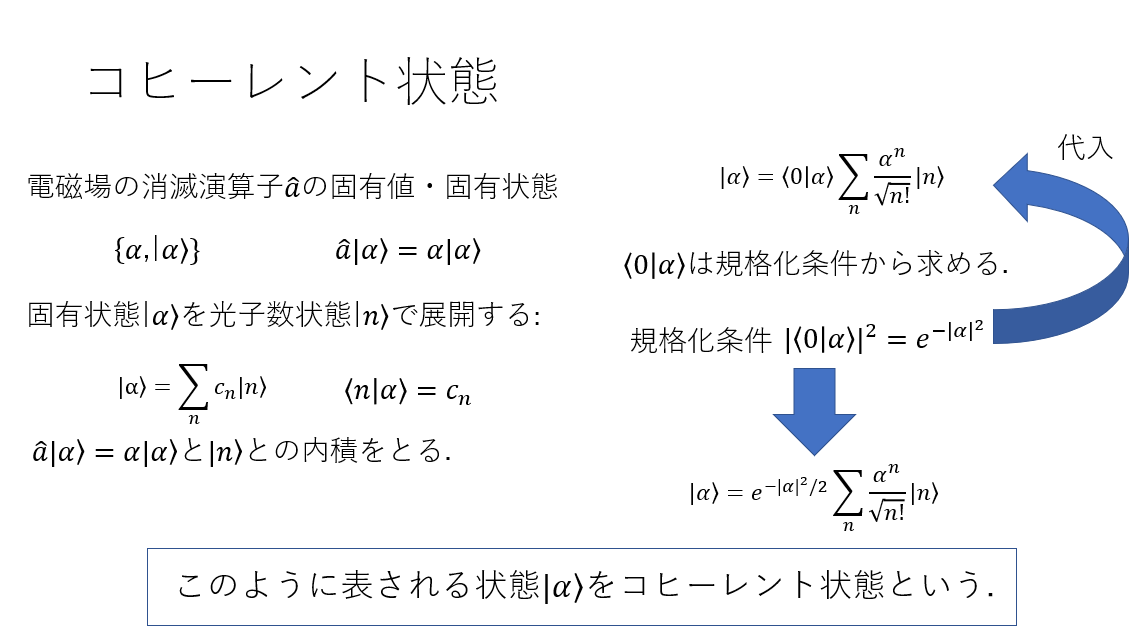
\includegraphics[width=0.5\textwidth]{img/zemi9.png}
        \caption[sample image (png)]{コヒーレント状態.}
        \label{Fig:1_5_1}
    \end{figure}
    
    \figref{Fig:1_5_1}はコヒーレント状態の定義を表している.コヒーレント状態は電磁場の消滅演算子の固有状態として与えられる.
    
\begin{figure}[htbp]
        \centering   
        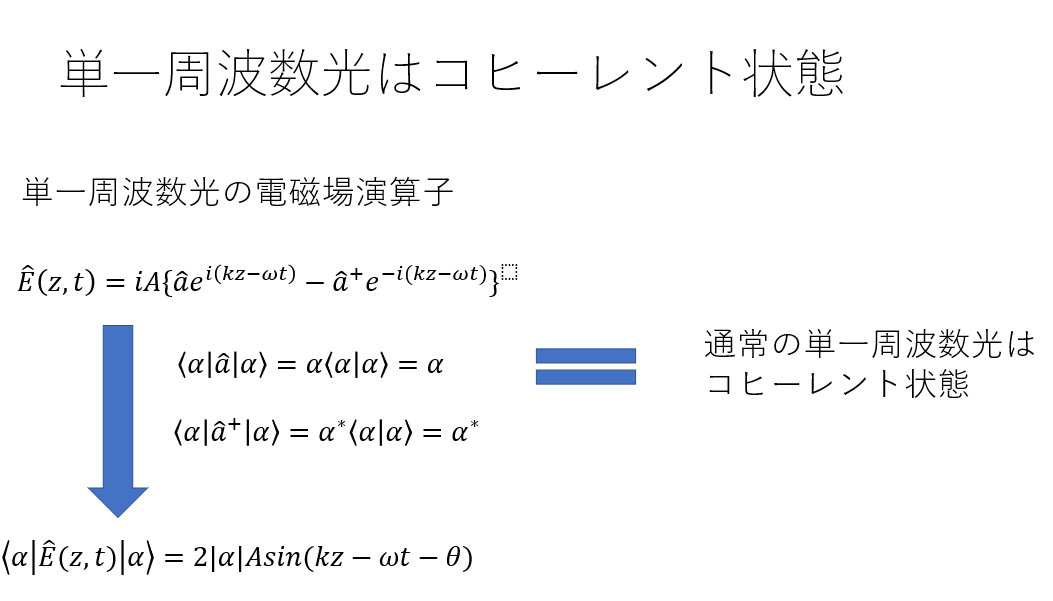
\includegraphics[width=0.5\textwidth]{img/zemi10.png}
        \caption[sample image (png)]{単一周波数光はコヒーレント状態.}
        \label{Fig:1_5_2}
    \end{figure}
    
    \figref{Fig:1_5_2}に示すように通常の単一周波数光はコヒーレント状態としてあらわされる.

\begin{figure}[htbp]
        \centering   
        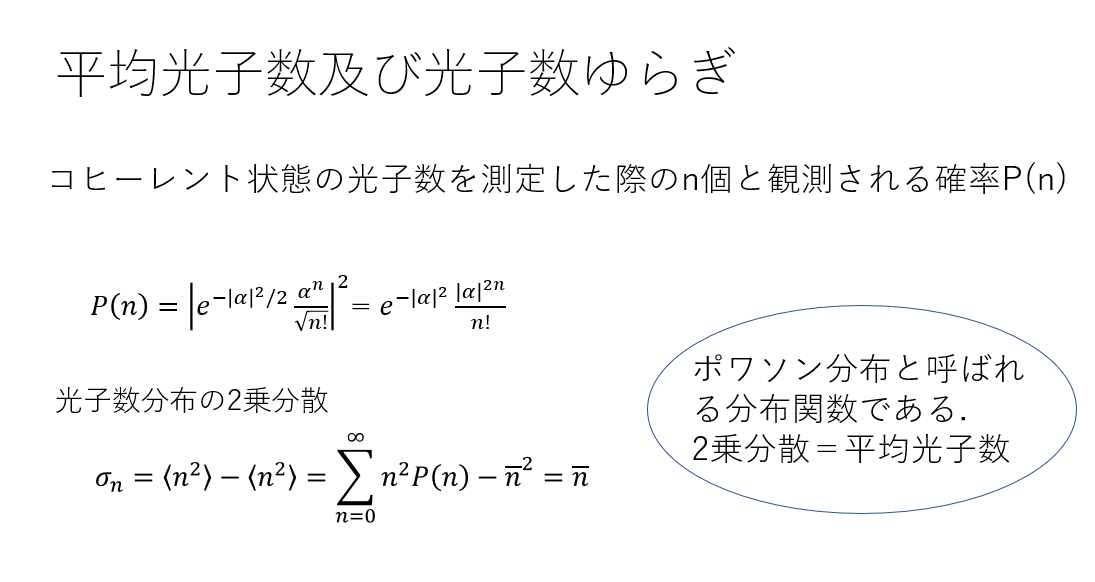
\includegraphics[width=0.5\textwidth]{img/zemi11.png}
        \caption[sample image (png)]{平均光子数及び光子数ゆらぎ.}
        \label{Fig:1_5_3}
    \end{figure}
    
    \figref{Fig:1_5_3}はコヒーレント状態の光子数を測定した際の$n$個と観測される確率$P(n)$について説明している.$P(n)$はポワソン分布と呼ばれる分布関数である.

\begin{figure}[htbp]
        \centering   
        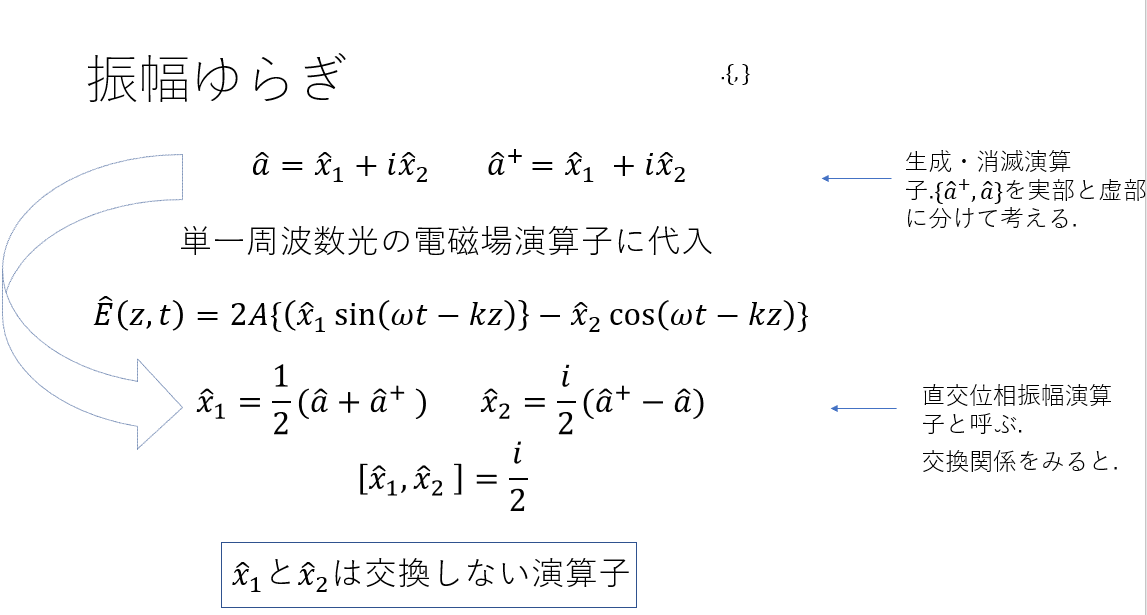
\includegraphics[width=0.5\textwidth]{img/zemi12.png}
        \caption[sample image (png)]{振幅ゆらぎ.}
        \label{Fig:1_5_4}
    \end{figure}

    \figref{Fig:1_5_4}は複素振幅の実部と虚部を表す演算子($\hat{x_1}$),($\hat{x_2}$)の交換関係について説明している.

\begin{figure}[htbp]
        \centering   
        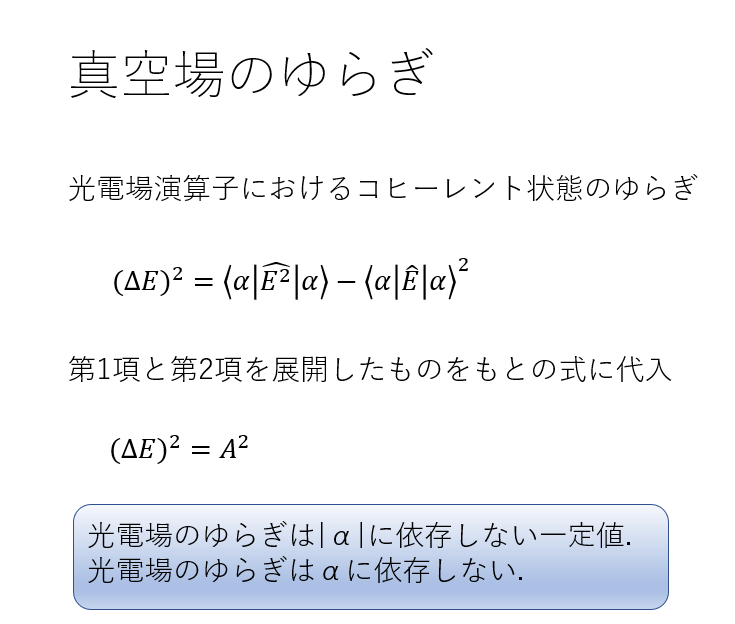
\includegraphics[width=0.5\textwidth]{img/zemi13.png}
        \caption[sample image (png)]{真空場のゆらぎ.}
        \label{Fig:1_5_5}
    \end{figure}
    \figref{Fig:1_5_5}は真空場のゆらぎについて説明しているこのゆらぎは$α$に依存しない.
    
\begin{figure}[htbp]
        \centering   
        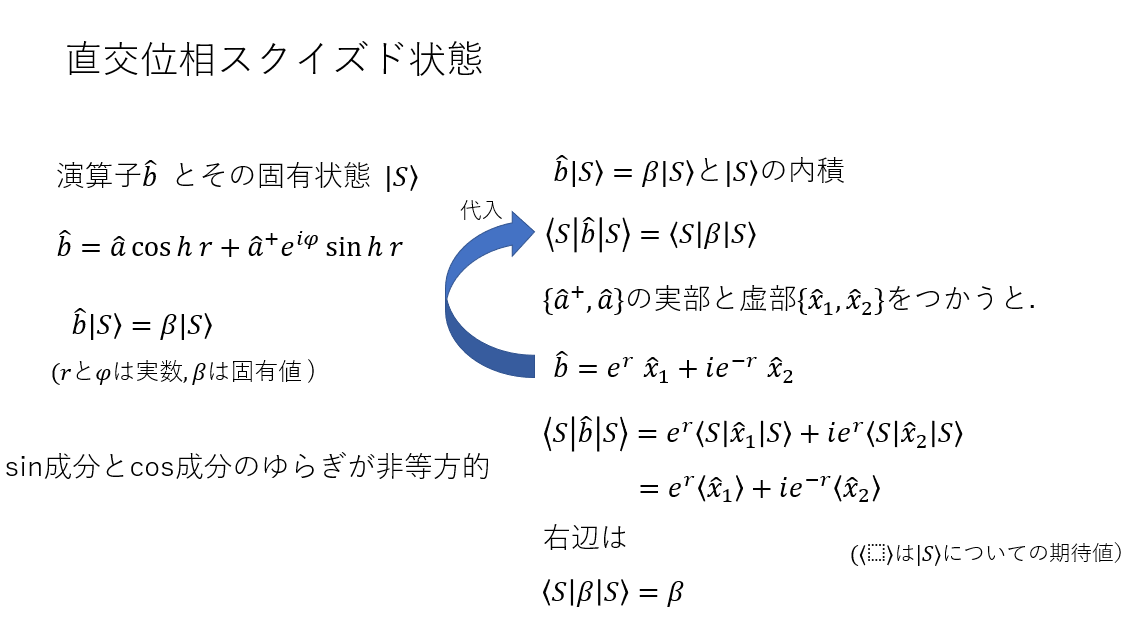
\includegraphics[width=0.5\textwidth]{img/zemi14.png}
        \caption[sample image (png)]{直交スクイズド状態.}
        \label{Fig:1_5_6}
    \end{figure}
    \figref{Fig:1_5_6}はスクイズド状態について説明している.直交位相スクイズド状態は演算子($\hat{b}$)とその固有状態$|{S}\rangle$として与えられる.

\section{光の状態
}
\begin{figure}[htbp]
        \centering   
        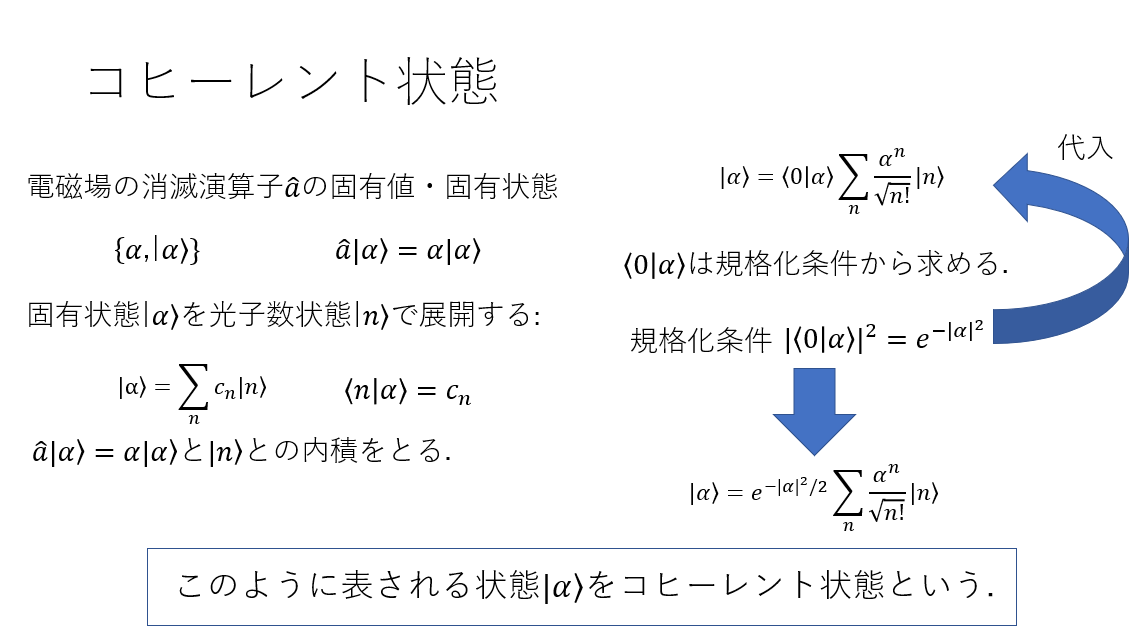
\includegraphics[width=0.5\textwidth]{img/zemi9.png}
        \caption[sample image (png)]{コヒーレント状態.}
        \label{Fig:1_5_1}
    \end{figure}
    
    \figref{Fig:1_5_1}はコヒーレント状態の定義を表している.コヒーレント状態は電磁場の消滅演算子の固有状態として与えられる.
    
\begin{figure}[htbp]
        \centering   
        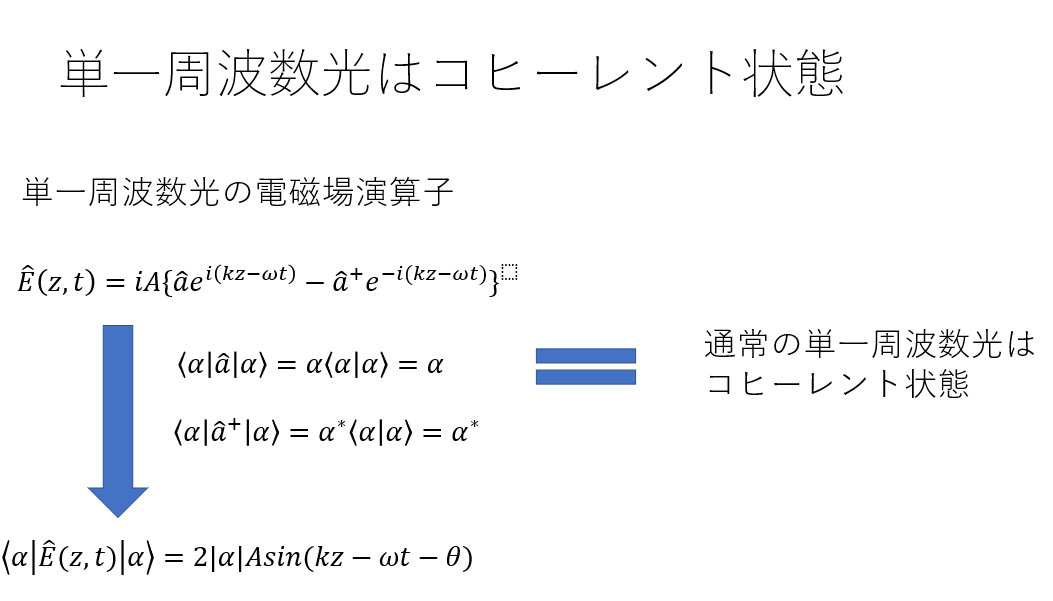
\includegraphics[width=0.5\textwidth]{img/zemi10.png}
        \caption[sample image (png)]{単一周波数光はコヒーレント状態.}
        \label{Fig:1_5_2}
    \end{figure}
    
    \figref{Fig:1_5_2}に示すように通常の単一周波数光はコヒーレント状態としてあらわされる.

\begin{figure}[htbp]
        \centering   
        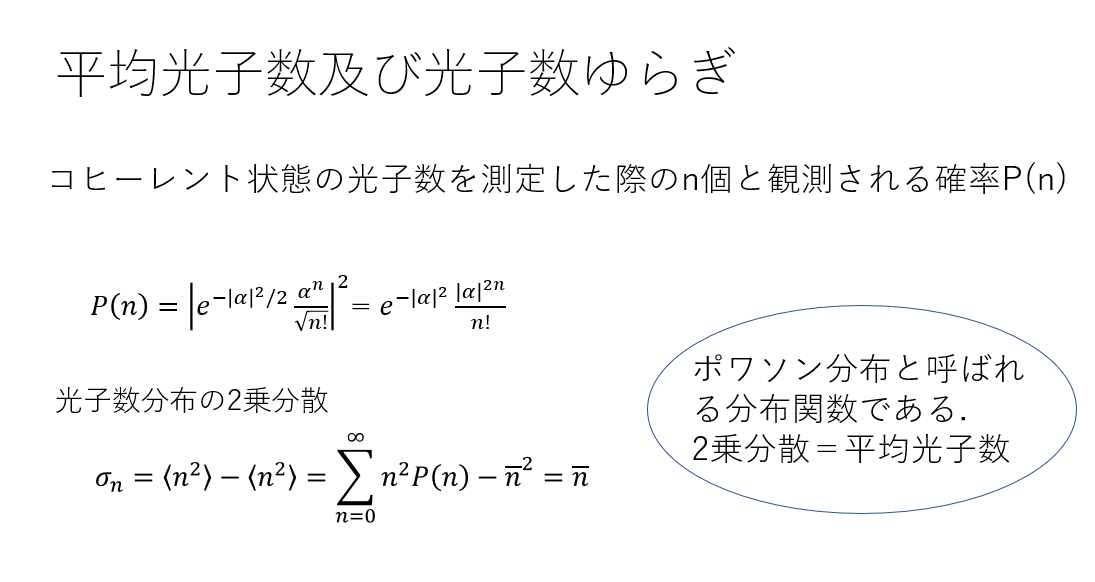
\includegraphics[width=0.5\textwidth]{img/zemi11.png}
        \caption[sample image (png)]{平均光子数及び光子数ゆらぎ.}
        \label{Fig:1_5_3}
    \end{figure}
    
    \figref{Fig:1_5_3}はコヒーレント状態の光子数を測定した際の$n$個と観測される確率$P(n)$について説明している.$P(n)$はポワソン分布と呼ばれる分布関数である.

\begin{figure}[htbp]
        \centering   
        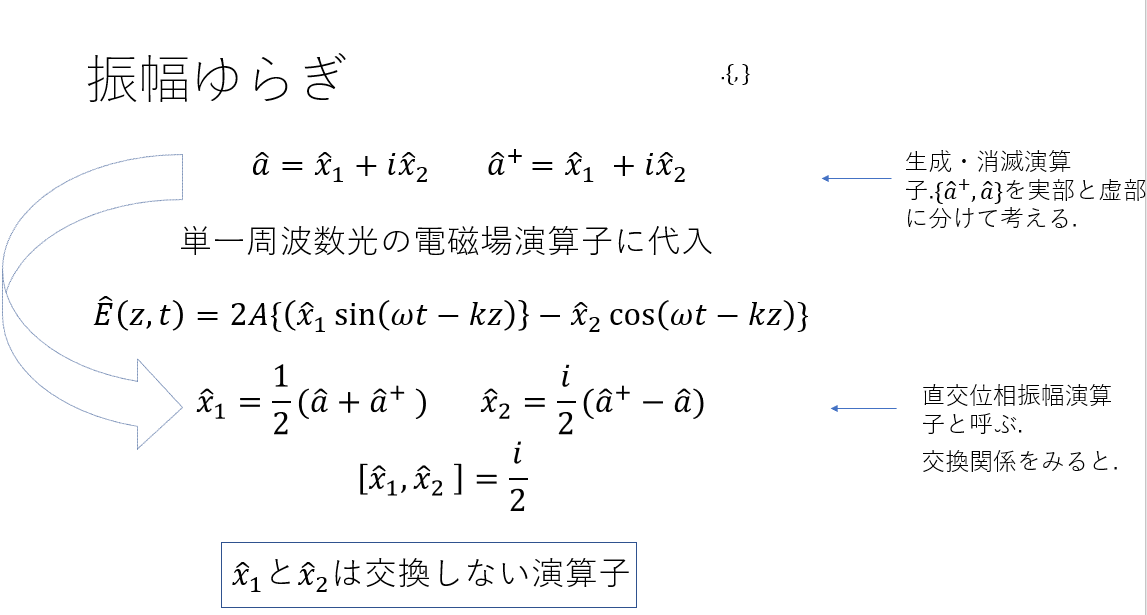
\includegraphics[width=0.5\textwidth]{img/zemi12.png}
        \caption[sample image (png)]{振幅ゆらぎ.}
        \label{Fig:1_5_4}
    \end{figure}

    \figref{Fig:1_5_4}は複素振幅の実部と虚部を表す演算子($\hat{x_1}$),($\hat{x_2}$)の交換関係について説明している.

\begin{figure}[htbp]
        \centering   
        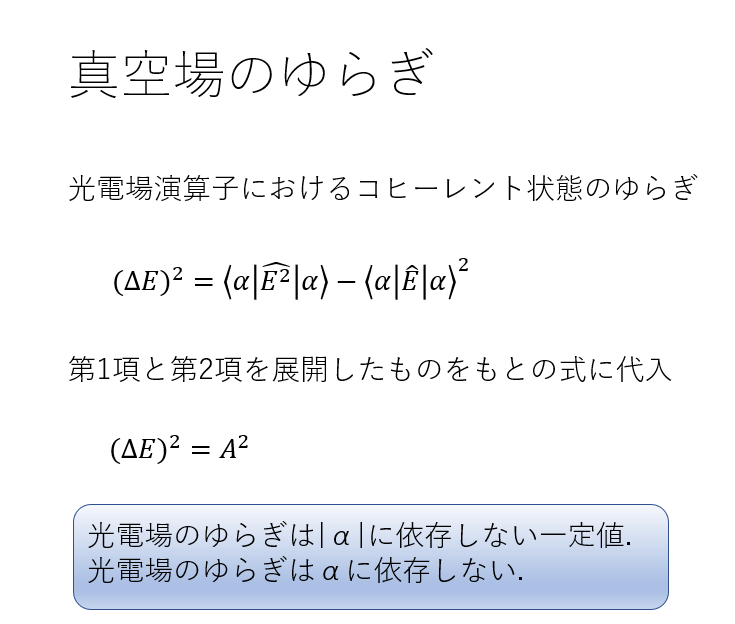
\includegraphics[width=0.5\textwidth]{img/zemi13.png}
        \caption[sample image (png)]{真空場のゆらぎ.}
        \label{Fig:1_5_5}
    \end{figure}
    \figref{Fig:1_5_5}は真空場のゆらぎについて説明しているこのゆらぎは$α$に依存しない.
    
\begin{figure}[htbp]
        \centering   
        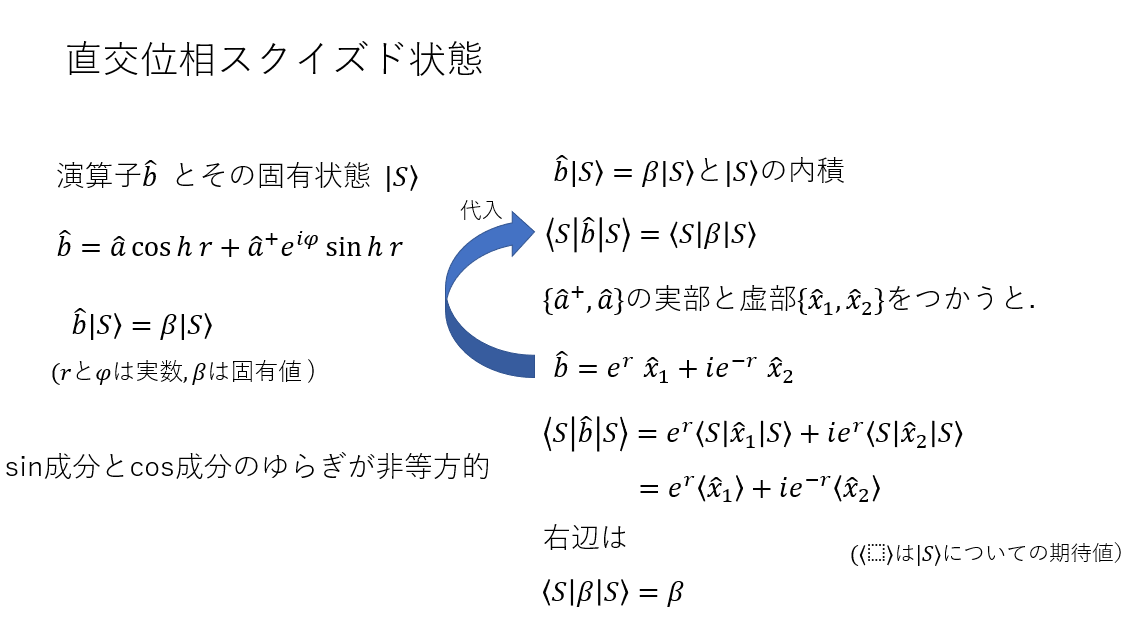
\includegraphics[width=0.5\textwidth]{img/zemi14.png}
        \caption[sample image (png)]{直交スクイズド状態.}
        \label{Fig:1_5_6}
    \end{figure}
    \figref{Fig:1_5_6}はスクイズド状態について説明している.直交位相スクイズド状態は演算子($\hat{b}$)とその固有状態$|{S}\rangle$として与えられる.
    
\section{Y00-量子暗号の信号状態
}
まず,コヒーレント状態について説明する.コヒーレント状態は,複素振幅$\alpha=x+iy$を持つ理想的なレーザー光を表す量子状態である.コヒーレント状態の複素振幅$\alpha$は複素平面上で平均$(x,y)^T$,共分散行列 
$$
\begin{pmatrix}
1/4&0\\
0&1/4
\end{pmatrix}
$$
の正規分布に従って揺らいでいる.\figref{Fig:3_1}は,平均$(x,y)^T$のコヒーレント状態の揺らぎを表している.

\begin{figure}[htbp]
        \centering   
        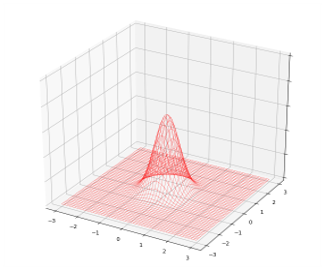
\includegraphics[width=0.5\textwidth]{img/zemi1.png}
        \caption[sample image (png)]{コヒーレント状態のゆらぎ}
        \label{Fig:3_1}
    \end{figure}
    



Y00-量子暗号の信号状態について説明する.青い丸がコヒーレント状態でこれを使って通信を行う.使用する基底によって0と1に対応する信号状態が異なる.例えば基底1を使って0を送りたいときは0のコヒーレント状態を使い,1を送りたいときは0のコヒーレント状態を使う.正規の受信者と送信者はどの基底を使って通信をしているのかわかる.同じ基底のコヒーレント状態は離れているので盗聴されにくいため,安全性が保証される.$S_{max}$は信号の最大強度を表している.$B$個の規定で通信する場合間隔の個数が$2B-1$個となることから隣接信号間の間隔は$S_{max}/2B-1$になる.このことから基底$k$の信号状態は

$$
\left |\frac{S_{max}}{2B-1}\right\rangle,\left |\frac{S_{max}}{2B-1}(B+k)\right\rangle
$$

\begin{figure}[htbp]
        \centering   
        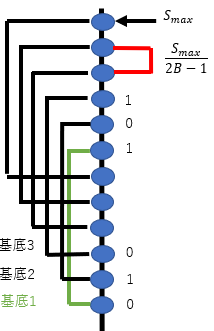
\includegraphics[width=0.5\textwidth]{img/zemi2.png}
        \caption[sample image (png)]{量子暗号の信号状態.}
        \label{Fig:3_2}
    \end{figure}
    
\section{Y00-量子暗号システム}
Y00-量子暗号のシステムについて説明する.送信者と受信者はseedkeyを共有している.まずLFSRによって疑似乱数を発生させる.
このとき,seedkeyが同じであるので発生する乱数も同じとなる.乱数は基底番号を表し,送信者と受信者は同じ基底番号を使うことができる.送信器では送信バイナリデータと基底番号の値に対応する量子状態を送信する.受信器では受け取った量子状態と基底番号を使ってバイナリデータを出力する.次に受信機における処理について説明する.

\begin{figure}[htbp]
        \centering   
        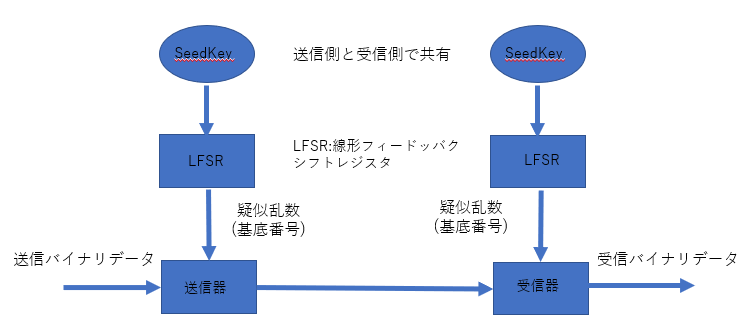
\includegraphics[width=0.5\textwidth]{img/zemi3.png}
        \caption[sample image (png)]{量子暗号システム.}
        \label{fig:4_1}
    \end{figure}



受信器ではまずホモダイン測定を行う.ホモダイン測定はコヒーレント状態の複素振幅$\alpha=x+iy$成分を測定する.\figref{Fig:4_2}は0と1に対応するコヒーレント状態をホモダイン測定した場合の出力の確率分布である.それぞれの分布は分散1/4の正規分布になっている.受信器では,測定値に基づき,しきい値を使って受信したデータが0か1か判断する.

\begin{figure}[htbp]
        \centering   
        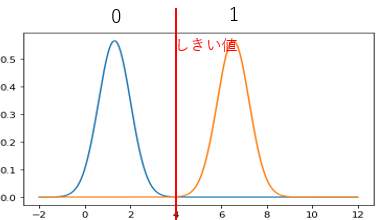
\includegraphics[width=0.5\textwidth]{img/zemi4}
        \caption[sample image (png)]{ホモダイン測定.}
        \label{Fig:4_2}
    \end{figure}
    
\figref{Fig:4_3}は受信機のしきい値処理を説明したものである.2つのコヒーレント状態の値のちょうど真ん中をしきい値とする.基底番号が3の場合それに対応するコヒーレント状態は緑色に示したコヒーレント状態になるが,そのときのしきい値は$\frac{S_{max}}{2B-1}(\frac{B}{2}+k)$となる.また,基底番号が奇数の場合,測定値がしきい値より大きければ1,小さければ0と判定する.基底番号が偶数の場合,測定値がしきい値より大きければ0,小さければ1と判定する.

\begin{figure}[htbp]
        \centering   
        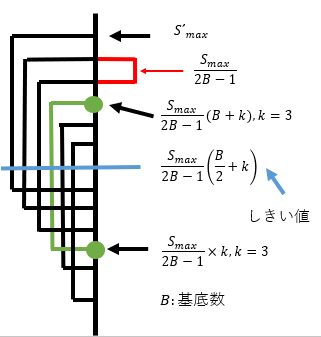
\includegraphics[width=0.5\textwidth]{img/zemi5.png}
        \caption[sample image (png)]{受信機のしきい値処理.}
        \label{Fig:4_3}
    \end{figure}
    
\section{通信路に減衰がある場合}
今回の評価実験では通信路が減衰の影響を受ける場合について考える.
\figref{Fig:5_1}は減衰の影響について表した.
減衰を受けることにより,平均$\mu$は$\sqrt{k}\mu$となる.
また,共分散行列$A$は,$kA+ (1-k)/4 $となる.ここで,$k$は透過率を表す.ただし,コヒーレント状態の場合,共分散行列は減衰によって変化しない.


\begin{figure}[htbp]
        \centering   
        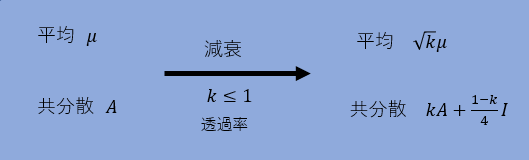
\includegraphics[width=0.5\textwidth]{img/zemi6.png}
        \caption[sample image (png)]{減衰の影響.}
        \label{Fig:5_1}
    \end{figure}





\figref{Fig:5_2}は,今回の評価実験の構成図になる.この通信路が透過率$k$の減衰の影響を受けている.
ここで,送信器の信号の最大強度の設定を$S_{max}$,受信機の信号の最大強度の設定を$S'_{max}$とする.
実験では$S_{max}$と$S´_{max}$が等しい場合と減衰の効果を考慮して$S´_{max}$を決める場合について実験を行った.
また,今回の実験では受信器は乱数を発生させてシミュレートした.
\begin{figure}[H]
        \centering   
        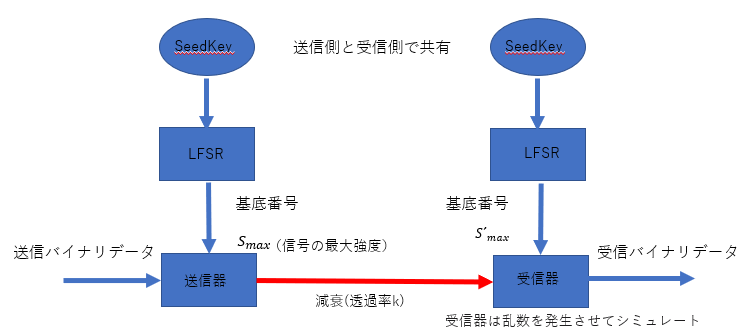
\includegraphics[width=0.5\textwidth]{img/zemi7.png}
        \caption[sample image (png)]{減衰がある場合の正規受信者の誤り率.}
        \label{Fig:5_2}
    \end{figure}


\section{評価実験}
減衰がある場合の正規受信者の誤り率を評価する.以下は送信者側のプログラムである.



\figref{Fig:5_3}は信号の最大強度が5,基底数が256,送信データ数が1000個の場合に透過率と正規受信者の誤り率の関係を表したものである.また,縦軸は誤り率,横軸は透過率で,透過率を0〜0.05づつ1.0まで上げた際の変化をまとめた.グラフからわかる通り,信号の最大強度を調整することで,0.05〜0.6の間で誤り率を大幅に減らすことができることがわかる.また透過率が0.8~1.0の範囲では信号の最大強度を調整しなくても信号の誤り率が低くなることがわかる.
\begin{figure}[htbp]
        \centering   
        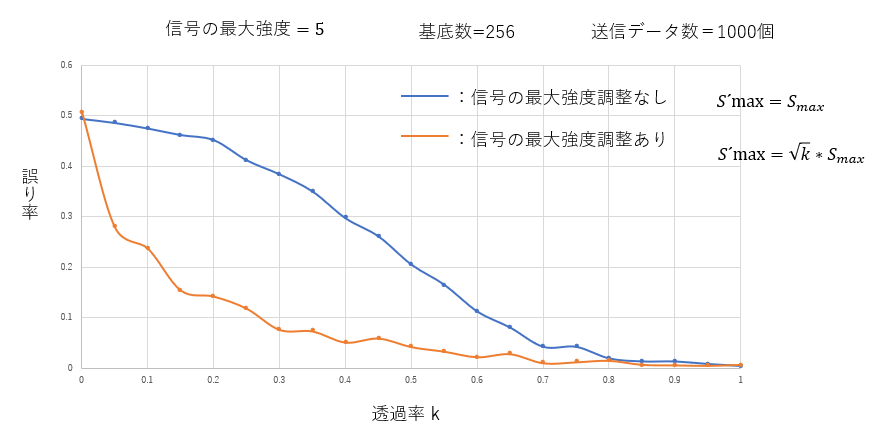
\includegraphics[width=0.5\textwidth]{img/zemi8.png}
        \caption[sample image (png)]{透過率と正規受信者の誤り率の関係.}
        \label{Fig:5_3}
    \end{figure}

\section{章タイトル}
コヒーレント状態$|\alpha\rangle$は,理想的なレーザー光を表している量子状態で,複素振幅$\alpha=x+iy$を持っている.また複素平面上で平均ベクトル$(x,y)^T$と共分散行列
$$
\begin{pmatrix}
1/4&0\\
0&1/4
\end{pmatrix}
$$
の正規分布に従って揺らいでいる.そしてコヒーレント状態を一般化したものが量子ガウス状態である.量子ガウス状態は,平均ベクトル$(x,y)^T$と共分散行列
$$
\begin{pmatrix}
a&c\\
c&b
\end{pmatrix}
$$
で表される.ただし共分散行列の要素は,関係式
$a+b\geq 0$,$ab-c^2\geq1/16$
を満たす必要がある.
スクイズド状態$|\alpha,\zeta\rangle$はガウス状態の一種で,図1のように量子揺らぎを持っている.スクイズド状態は,複素数$\alpha,\zeta$によって特徴づけられる.特に$\alpha$を$x+iy$,$\zeta$を$re^{i\theta}$とすると,
\begin{equation}
\begin{split}
a&=1/4[\cosh 2r-\sinh 2r\cos\theta]\\
b&=1/4[\cosh 2r+\sinh 2r\cos\theta]\\
c&=1/4\sinh 2r\sin\theta
\end{split}
\end{equation}
によって平均ベクトル$(x,y)^T$と共分散行列
\begin{equation}
\begin{pmatrix}
a&c\\
c&b
\end{pmatrix}
\end{equation}
が決まる.

図1:スクイズド状態
</center>
 



```python

```







\section{まとめ}



\begin{thebibliography}{9}
\bibitem{Futami}Fumio Futami and Osamu Hirota,Two Months Field
Transmission Test of 2.5-Gb/s Y-00 Cipher in 160-km (40 km x 4
spans)Installed Optical Fiber Cable for Secure Optical Fiber Communications,Tamagawa University Quantum ICT Research Institute Bulletin, Vol.2, No.1, 15-17, 2012 

\bibitem{久保}久保貴星,光通信量子暗号のシミュレーション, 玉川大学工学部情報通信工学科卒業論文, 2020 
\end{thebibliography}
\end{document}
